\documentclass[a4paper,11pt]{article}

\usepackage[ngerman]{babel}

\usepackage{url}
\usepackage{abstract}
\usepackage{graphicx}
\usepackage{booktabs}
\usepackage{float}
\usepackage{tabularx}
\usepackage{amsmath}
\usepackage{hyperref}
\usepackage{listings}
\usepackage{color}
\usepackage{xcolor}
\usepackage{todonotes}
\usepackage[binary-units]{siunitx}
\usepackage{hyphenat}
\usepackage{fontspec}
\usepackage{todonotes}
\usepackage{longtable}
\usepackage{booktabs}
\usepackage{rotating}
\usepackage{pdflscape}
\usepackage{caption}
\usepackage{makecell}
%%\usepackage[bottom]{footmisc} breaks referencing of footnotes idk

\usepackage{tgpagella}
\setmainfont{TeX Gyre Pagella}

\usepackage[top=3cm]{geometry}
\usepackage{parskip} %% Absatz anstatt amerikanischer Einrückung

% configure vertical spacing in lists
\usepackage{enumitem}
\setitemize{partopsep=4pt,parsep=2pt}
\setdescription{partopsep=4pt,parsep=6pt}

\makeatletter
\def\namedlabel#1#2{\begingroup
#2%
\def\@currentlabel{#2}%
\phantomsection\label{#1}\endgroup
}
\makeatother

\definecolor{dkgreen}{rgb}{0,0.6,0}
\definecolor{gray}{rgb}{0.5,0.5,0.5}
\definecolor{mauve}{rgb}{0.58,0,0.82}

\lstdefinelanguage[postgres]{SQL}[]{SQL}{
    morekeywords={SERIAL, BYTEA, BOOLEAN},
}
\lstset{
    numbers=none,
    language=[postgres]SQL,
    frame=tb,
    captionpos=below,
    aboveskip=3mm,
    belowskip=3mm,
    xleftmargin=.01\textwidth, xrightmargin=.01\textwidth,
    showstringspaces=false,
    columns=flexible,
    basicstyle={\small\ttfamily},
    numberstyle=\tiny\color{gray},
    keywordstyle=\color{blue},
    commentstyle=\color{dkgreen},
    stringstyle=\color{mauve},
    breaklines=false,
    breakatwhitespace=true,
    tabsize=4
}

\newcommand{\shellcmd}[1]{\texttt{\footnotesize\$ #1}}

\newcommand{\localauthor}[1]{\color{gray} #1 \normalcolor}

\newcommand{\XXitem}[2]{\item[] \textbf{#1} \phantomsection \label{#2}}

\newcommand{\phantomLabel}[1]{\phantomsection\label{#1}}

\newcommand{\doubletitle}[2]{\title{#1 \\ [1ex] \normalsize #2}}
\newcommand{\extauthor}[2]{\author{#1 \\ \normalsize #2}}
\newcommand{\code}[1]{\texttt{#1}}

\begin{document}

    \begin{titlepage}
        \centering

        $~$

        \vspace{0.2cm} %% Hack for vspace to work

        \Huge \textbf{Implementierungsplan}\\

        \Huge Team 2
        \Large

        SEP WS 2021/22

        \vspace{2cm}

        
\includegraphics[width=0.8\linewidth]{graphics/LasEs-logo}

        \vspace{2cm}

        Betreuer:

        \textsc{Prof. Dr. Christian Bachmaier}

        \vspace{1cm}

        \begin{table}[H]
            \centering
            \Large
            \begin{tabular}{ll}
                \toprule
                \textbf{Projektphase} & \textbf{Leiter} \\
                \midrule
                Pflichtenheft & Johann Schicho \\
                Entwurf & Stefanie Gürster \\
                Feinspezifikation & Johannes Garstenauer \\
                Implementierung & Thomas Kirz \\
                Validierung & Sebastian Vogt \\
                \bottomrule
            \end{tabular}
        \end{table}

        \vspace{1cm}

        3. Dezember 2021

    \end{titlepage}

    \pagenumbering{gobble}

    %%\maketitle
    \tableofcontents
    %%\listoftodos

    %% ENDE Titelblatt

    \newpage
    \pagenumbering{arabic}

    \section{Einleitung}\label{sec:einleitung}
    \localauthor{Thomas Kirz}

LasEs ist ein \emph{Submission und Review Management System}, also eine Webseite bei der Wissenschaftler:innen Artikel hochladen können, um von Gutachtern \emph{peer reviewed} zu werden.\\
Auf Basis der Gutachten kann ein \emph{Editor} eines Journals oder einer Konferenz den Artikel für die Veröffentlichung akzeptieren.


    \section{Arbeitspakete}\label{sec:arbeitspakete}
    \subsection{Milestone 1}
\localauthor{Stefanie Gürster}

\subsection{Milestone 2}
\localauthor{Sebastian Vogt}

\subsection{Milestone 3}
\localauthor{Johannes Garstenauer}

    \section{Abhängigkeiten}\label{sec:abhaengigkeiten}
    \localauthor{Thomas Kirz}

Abbildung~\ref{fig:pert} zeigt alle Arbeitspakete mit ihrem Bearbeiter und dem geschätzten Zeitaufwand
und stellt eine Übersicht über die Abhängigkeiten zwischen den Paketen dar.
Es kann oft trotz einer Abhängigkeit zwischen zwei Arbeitspaketen gleichzeitig mit beiden begonnen werden,
dies wird durch eine gestrichelte Linien gekennzeichnet.

\begin{figure}
    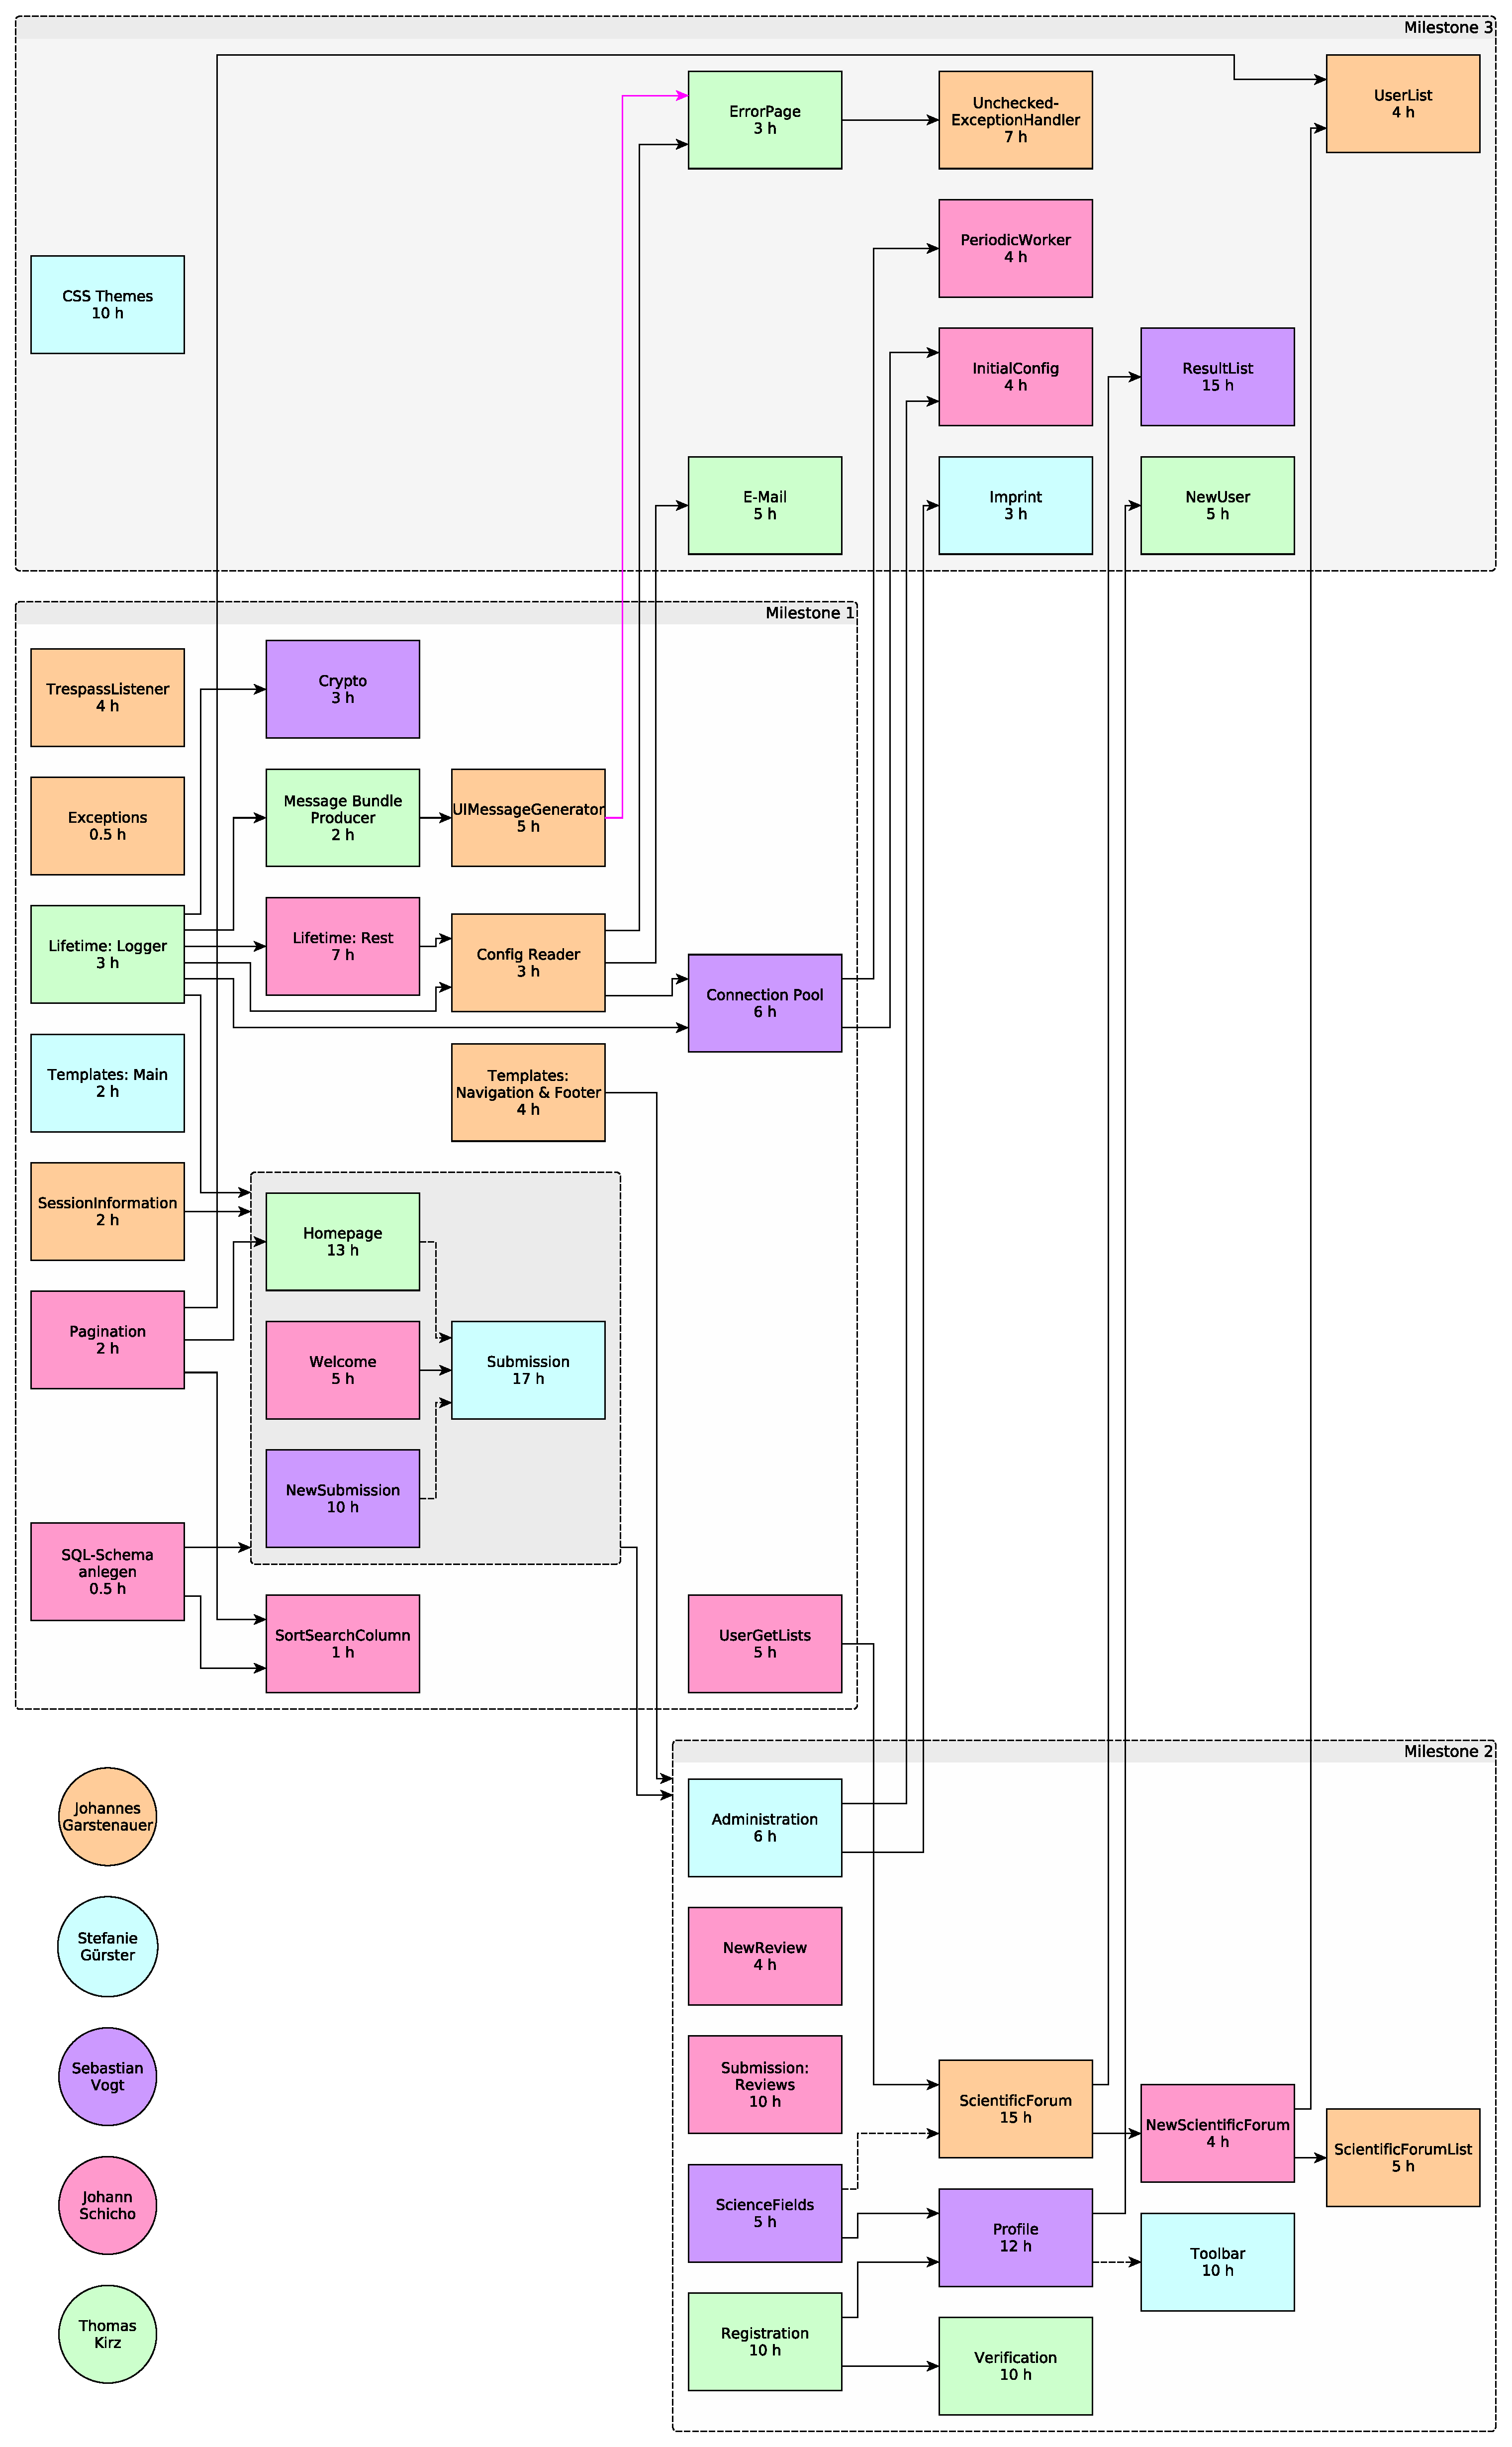
\includegraphics[width=\textwidth]{graphics/pert}
    \caption{Abhängigkeiten der Arbeitspakete in einem PERT-Chart}
    \label{fig:pert}
\end{figure}

    \section{Spezialgebiete}\label{sec:spezialgebiete}
    \localauthor{Johann Schicho}
    \newpage
    \section{Tests}\label{sec:tests}
    \lstset{
    language=Java,
    basicstyle=\ttfamily\selectfont\scriptsize,
}

\newcommand{\testlisting}[1]{\lstinputlisting[label={lst:#1},caption={#1.java}]{tests/#1.java}}

Es folgen Beispiele für Whitebox-Tests für verschiedene Arbeitspakete aus allen Milestones.
Sie sollen repräsentativ sein für bei der Implementierung entstehende Tests, sind aber nicht zwingend vollständige
Test-Suites für die jeweiligen Klassen oder Arbeitspakete.

\subsection{Milestone 1}\label{subsec:milestone1}

\subsubsection{Arbeitspaket \emph{Submission}}
\localauthor{Thomas Kirz}
\testlisting{SubmissionBackingTest}
\testlisting{SubmissionServiceTest}
\testlisting{SubmissionRepositoryTest}

\subsubsection{Arbeitspaket \emph{Welcome}}
\localauthor{Johann Schicho}
\testlisting{LoginServiceTest}

<<<<<<< HEAD
\subsubsection{UserGetLists}
\localauthor{Johann Schicho}
\testlisting{UserRepositoryGetListTest}
=======
\subsubsection{Arbeitspaket \emph{Connection Pool}}
\localauthor{Sebastian Vogt}
\testlisting{TransactionTest}
>>>>>>> f3cb1703bc0ae81331b09a6d2f54db3117640463

\subsection{Milestone 2}\label{subsec:milestone2}

\subsubsection{Arbeitspaket \emph{Registration}}
\localauthor{Thomas Kirz}
\testlisting{PasswordValidatorTest}
\testlisting{RegistrationServiceTest}
\testlisting{UserRepositoryTest}

\subsubsection{Arbeitspaket \emph{Profile}}
\localauthor{Johann Schicho}
\testlisting{ProfileBackingTest}
\subsection{Milestone 3}\label{subsec:milestone3}

\subsubsection{Arbeitspaket \emph{ErrorPage}}
\testlisting{ErrorPageBackingTest}
\testlisting{ErrorMessageTest}

\subsubsection{Arbeitspaket \emph{Email}}
\localauthor{Johann Schicho}
\testlisting{EmailUtilTest}


\end{document}
